% ========================================
% CAPÍTULO 4: PROTOCOLO DE VALIDACIÓN, LÍNEA BASE Y RESULTADOS PRELIMINARES  (criterio 4)
% ========================================

\chapter{VALIDACIÓN, LÍNEA BASE Y RESULTADOS PRELIMINARES}
\label{ch:validacion}

\section{Protocolo para evitar la fuga en la propia evaluación}

Se aplica al experimento lo que se audita: (i) validación cruzada de 5 pliegues (estratificada en clasificación) con semilla 42 y los \textbf{mismos pliegues} para \texttt{leaky} y \texttt{clean}; (ii) en la versión \texttt{clean} y en el código reparado, todo el preprocesamiento va dentro de un \texttt{Pipeline}, de modo que se ajusta solo con el entrenamiento de cada pliegue; (iii) el verificador en ejecución comprueba que, en \texttt{clean}, ningún transformador vea tantas filas como el total (el máximo observado es 80,3\,\%); (iv) las pruebas estadísticas usan como unidad el \textbf{par} (dataset $\times$ tipo de fuga) y no los pliegues, que no son independientes.

\section{Métricas y líneas base}

Las métricas se derivan de los criterios de éxito (Tabla~\ref{tab:exito}). \emph{Del auditor} (positivo = «hay fuga»): precisión, recall, F1 y valor predictivo negativo (VPN), porque el error más costoso es declarar limpio un script con fuga (falsa seguridad); el recall de la evaluación independiente se acompaña de un intervalo exacto de Clopper--Pearson \parencite{clopper1934}, adecuado para muestras pequeñas. \emph{Del daño}: \DOpt{} en ROC-AUC (clasificación, insensible al umbral y al desbalance) y $R^2$ (regresión, comparable entre datasets), con F1 macro y RMSE como secundarias; la media de \DOpt{} por familia se informa con un intervalo bootstrap percentil del 95\,\% \parencite{efron1993}.

Se definen tres líneas base, cada una como punto de comparación de una afirmación distinta:
\begin{itemize}
  \item \textbf{Del daño:} el pipeline \texttt{clean}. Es el desempeño que se habría reportado sin el error, por lo que \DOpt{} mide exactamente el exceso atribuible a la fuga.
  \item \textbf{Del detector híbrido:} cada componente por separado (solo AST y solo ejecución). Justifica que combinar ambos aporte algo.
  \item \textbf{Externa:} una regla trivial (\arch{baseline_simple_rule.py}) que declara fuga si el script ajusta un transformador con \texttt{.fit} y no usa ningún \texttt{Pipeline}, ignorando comentarios e importaciones. Representa lo que haría un revisor apurado con una búsqueda de texto; si el auditor no la supera, su complejidad no se justifica. La escribió el autor y no es un \emph{linter} de terceros; la comparación con un LLM juez queda para Capstone~II.
\end{itemize}

\section{Resultados: eficacia del auditor}
\label{sec:eficacia}

\begin{table}[!htbp]
\centering
\caption{Banco de control: 192 scripts con verdad conocida.}
\label{tab:banco}
\begingroup\footnotesize\singlespacing
\begin{tabular}{@{}l r r r r r r r@{}}
\toprule
Detector & TP & TN & FP & FN & Precisión & Recall & VPN \\
\midrule
AST (estático) & 96 & 96 & 0 & 0 & 1,00 & 1,00 & 1,00 \\
Ejecución & 96 & 96 & 0 & 0 & 1,00 & 1,00 & 1,00 \\
Híbrido & 96 & 96 & 0 & 0 & 1,00 & 1,00 & 1,00 \\
\bottomrule
\end{tabular}
\endgroup
\end{table}
\donde{TP, TN, FP, FN: verdaderos positivos, verdaderos negativos, falsos positivos y falsos negativos; $\mathrm{Precisión}=TP/(TP+FP)$; $\mathrm{Recall}=TP/(TP+FN)$; $\mathrm{VPN}=TN/(TN+FN)$.}

\textbf{Este 100\,\% no prueba que el auditor generalice}: el banco lo produce un generador escrito por el mismo autor que el auditor (evaluación circular), con patrones que este conoce. Por eso se añadió una \textbf{evaluación independiente} con 13 scripts escritos a mano (9 con fuga y 4 limpios), con estilos que el generador no produce: \texttt{make\_pipeline}, DataFrames, funciones auxiliares, alias de importación, variables \texttt{X\_te}, y \texttt{fit} y \texttt{transform} por separado.

\begin{table}[!htbp]
\centering
\caption{Evaluación independiente ($n=13$) y línea base externa (regla simple).}
\label{tab:indep}
\label{tab:base}
\begingroup\footnotesize\singlespacing
\begin{tabular}{@{}l l r r r r r c@{}}
\toprule
Conjunto & Detector & TP & FP & FN & Precisión & VPN & Recall [IC95\,\%] \\
\midrule
Independiente (13) & Regla simple & 8 & 1 & 1 & 0,89 & 0,75 & 0,89 [0,52; 1,00] \\
 & AST & 8 & 0 & 1 & 1,00 & 0,80 & 0,89 [0,52; 1,00] \\
 & Ejecución & 7 & 0 & 2 & 1,00 & 0,67 & 0,78 [0,40; 0,97] \\
 & Híbrido & 9 & 0 & 0 & 1,00 & 1,00 & 1,00 [0,66; 1,00] \\
\midrule
Banco (192) & Regla simple & 72 & 0 & 24 & 1,00 & 0,80 & 0,75 [0,65; 0,83] \\
 & Híbrido & 96 & 0 & 0 & 1,00 & 1,00 & 1,00 \\
\bottomrule
\end{tabular}
\endgroup
\end{table}
\nota{IC95\,\%: intervalo exacto de Clopper--Pearson para el recall. Conjunto independiente: 9 scripts con fuga y 4 limpios.}

La regla simple rinde sorprendentemente bien en los casos manuales (recall 0,89, igual que el AST), pero con un falso positivo (declara fuga en el script que escala \emph{después} de dividir) y deja pasar el alias de importación; en el banco pierde 24 de 96 fugas. El AST falla con el alias (\texttt{StandardScaler as SS}); la ejecución falla con ajustes que no usan todas las filas (el escalador re-ajustado con las filas de prueba y el ajustado con el 70\,\% de entrenamiento antes de la validación cruzada). Fallan en casos distintos, lo que respalda el diseño híbrido. Pero los intervalos se solapan ampliamente: con $n=9$ casos con fuga, el límite inferior del recall híbrido es 0,66, y la ventaja sobre la línea base es un margen que Capstone~II debe confirmar, no una mejora demostrada. La reparación automática resolvió 4 de los 9 scripts con fuga; en los otros 5 declaró «requiere revisión manual» y no tocó el código.

\section{Resultados preliminares: Sesgo de Optimismo}
\label{sec:dopt}

\begin{figure}[!htbp]
\centering
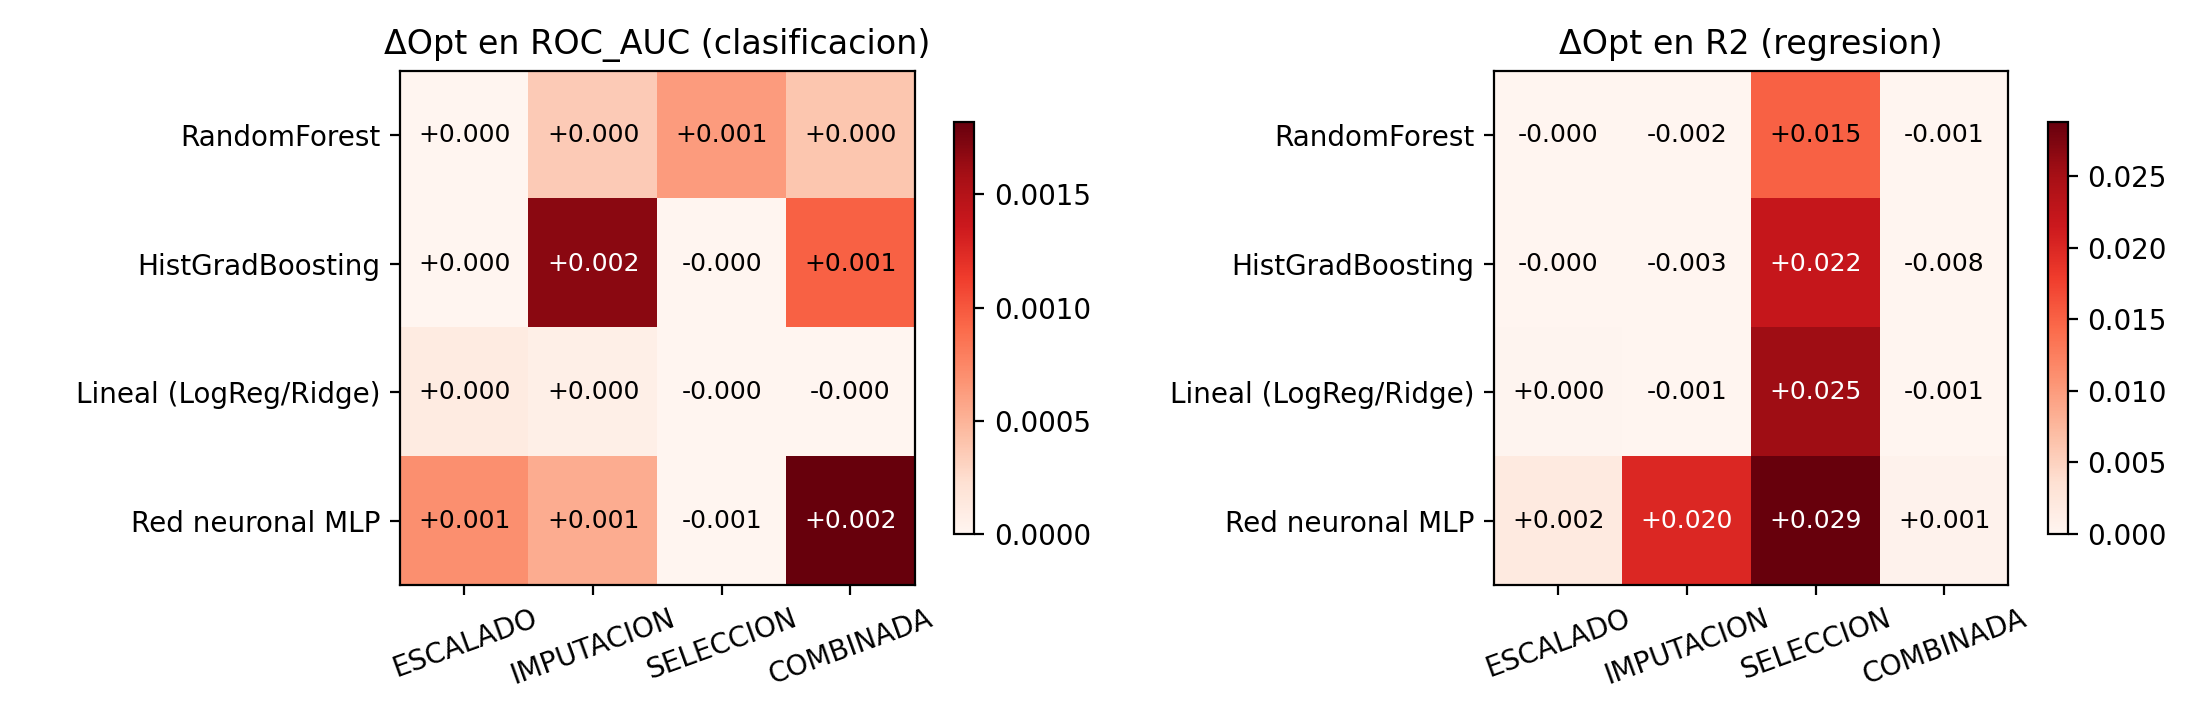
\includegraphics[width=0.88\textwidth]{fig_delta_opt_heatmap.png}
\caption{\DOpt{} medio por familia y tipo de fuga (ROC-AUC en clasificación, $R^2$ en regresión). El par degenerado (D5, MLP, combinada) está excluido.}
\label{fig:heatmap}
\end{figure}

\begin{table}[!htbp]
\centering
\caption{\DOpt{} medio, promedio sobre los datasets.}
\label{tab:dopt}
\begingroup\footnotesize\singlespacing
\begin{tabular}{@{}l l r r r r@{}}
\toprule
Tarea & Familia & Escalado & Imputación & Selección & Combinada \\
\midrule
Clasificación (AUC) & RandomForest & 0,0000 & 0,0004 & 0,0006 & 0,0004 \\
 & Gradient Boosting & 0,0000 & 0,0017 & $-0{,}0001$ & 0,0010 \\
 & Lineal & 0,0001 & 0,0001 & $-0{,}0001$ & 0,0000 \\
 & MLP & 0,0007 & 0,0005 & $-0{,}0009$ & 0,0018 \\
\midrule
Regresión ($R^2$) & RandomForest & $-0{,}0001$ & $-0{,}0024$ & 0,0150 & $-0{,}0014$ \\
 & Gradient Boosting & 0,0000 & $-0{,}0033$ & 0,0220 & $-0{,}0082$ \\
 & Lineal & 0,0001 & $-0{,}0008$ & 0,0255 & $-0{,}0007$ \\
 & MLP & 0,0019 & 0,0200 & 0,0288 & 0,0006$^{*}$ \\
\bottomrule
\end{tabular}
\endgroup
\end{table}
\nota{$^{*}$Media de 2 datasets (se excluyó el par degenerado).}

Se observan tres hechos. \textbf{(1) En clasificación, \DOpt{} es prácticamente nulo}: en 48 pares va de $-0{,}0027$ a $+0{,}0034$, con un AUC limpio mediano de 0,991 (efecto techo). \textbf{(2) En regresión aparece optimismo, concentrado en la selección con \texttt{california\_housing}}: $R^2$ de 0,690 (sin fuga) frente a 0,731 (con fuga) en RandomForest, y de 0,615 frente a 0,689 en MLP; en los 47 pares el rango es de $-0{,}023$ a $+0{,}074$. \textbf{(3) Escalado y árboles:} en RandomForest y HistGradientBoosting, en los 6 datasets, el máximo $|\DOpt|$ por escalado es 0,0002, como predice la teoría: una transformación afín creciente no cambia la estructura de un árbol.

\begin{table}[!htbp]
\centering
\caption{Pruebas por familia en regresión (fugas simples, $n=9$ pares).}
\label{tab:tests}
\begingroup\footnotesize\singlespacing
\begin{tabular}{@{}l r c r r r@{}}
\toprule
Familia & \DOpt{} medio & IC95\,\% bootstrap & $d$ de Cohen & $p$ Wilcoxon & $p$ Holm \\
\midrule
RandomForest & 0,0042 & [$-0{,}0023$; 0,0142] & 0,29 & 0,320 & 1,000 \\
Gradient Boosting & 0,0062 & [$-0{,}0021$; 0,0199] & 0,32 & 0,371 & 1,000 \\
Lineal (Ridge) & 0,0083 & [$-0{,}0015$; 0,0250] & 0,34 & 0,285 & 1,000 \\
MLP & 0,0169 & [0,0027; 0,0346] & 0,65 & \textbf{0,037} & 0,297 \\
\bottomrule
\end{tabular}
\endgroup
\end{table}
\nota{Hipótesis alternativa: $\DOpt>0$ (Wilcoxon unilateral). IC95\,\%: bootstrap percentil de la media con 10.000 remuestreos (semilla 42). $p$ Holm: ajuste de Holm sobre las 8 pruebas (2 tareas $\times$ 4 familias). Se usan las fugas simples porque la combinada repite esos mecanismos.}

En clasificación, el $p$ de Wilcoxon de todas las familias es $\geq 0{,}148$ y todos los intervalos incluyen el cero. En regresión, la MLP es la única familia cuyo intervalo excluye el cero y cuyo $p$ sin corregir es menor que 0,05, pero tras el ajuste de Holm \parencite{holm1979} su $p$ sube a 0,297. La prueba de Friedman entre familias da $p=0{,}84$ en clasificación y $p=0{,}041$ en regresión (rangos medios, donde 1 indica el mayor optimismo: RandomForest 3,39; Gradient Boosting 2,72; Lineal 2,11; MLP 1,78), que con la corrección de Bonferroni para dos pruebas pasa a 0,082. Por eso las diferencias entre familias se reportan como \textbf{exploratorias} \parencite{demsar2006}.

\section{Control positivo: cuándo la selección con fuga sí daña}
\label{sec:control}

Para comprobar que \DOpt{} detecta la fuga cuando esta importa, se repitió solo la selección con 0, 50, 200 y 1000 columnas de ruido, en dos escenarios: \emph{real} (etiquetas verdaderas) y \emph{señal nula} (etiquetas permutadas al azar, de modo que la verdad es AUC $=0{,}5$ y $R^2\leq 0$).

\begin{figure}[!htbp]
\centering
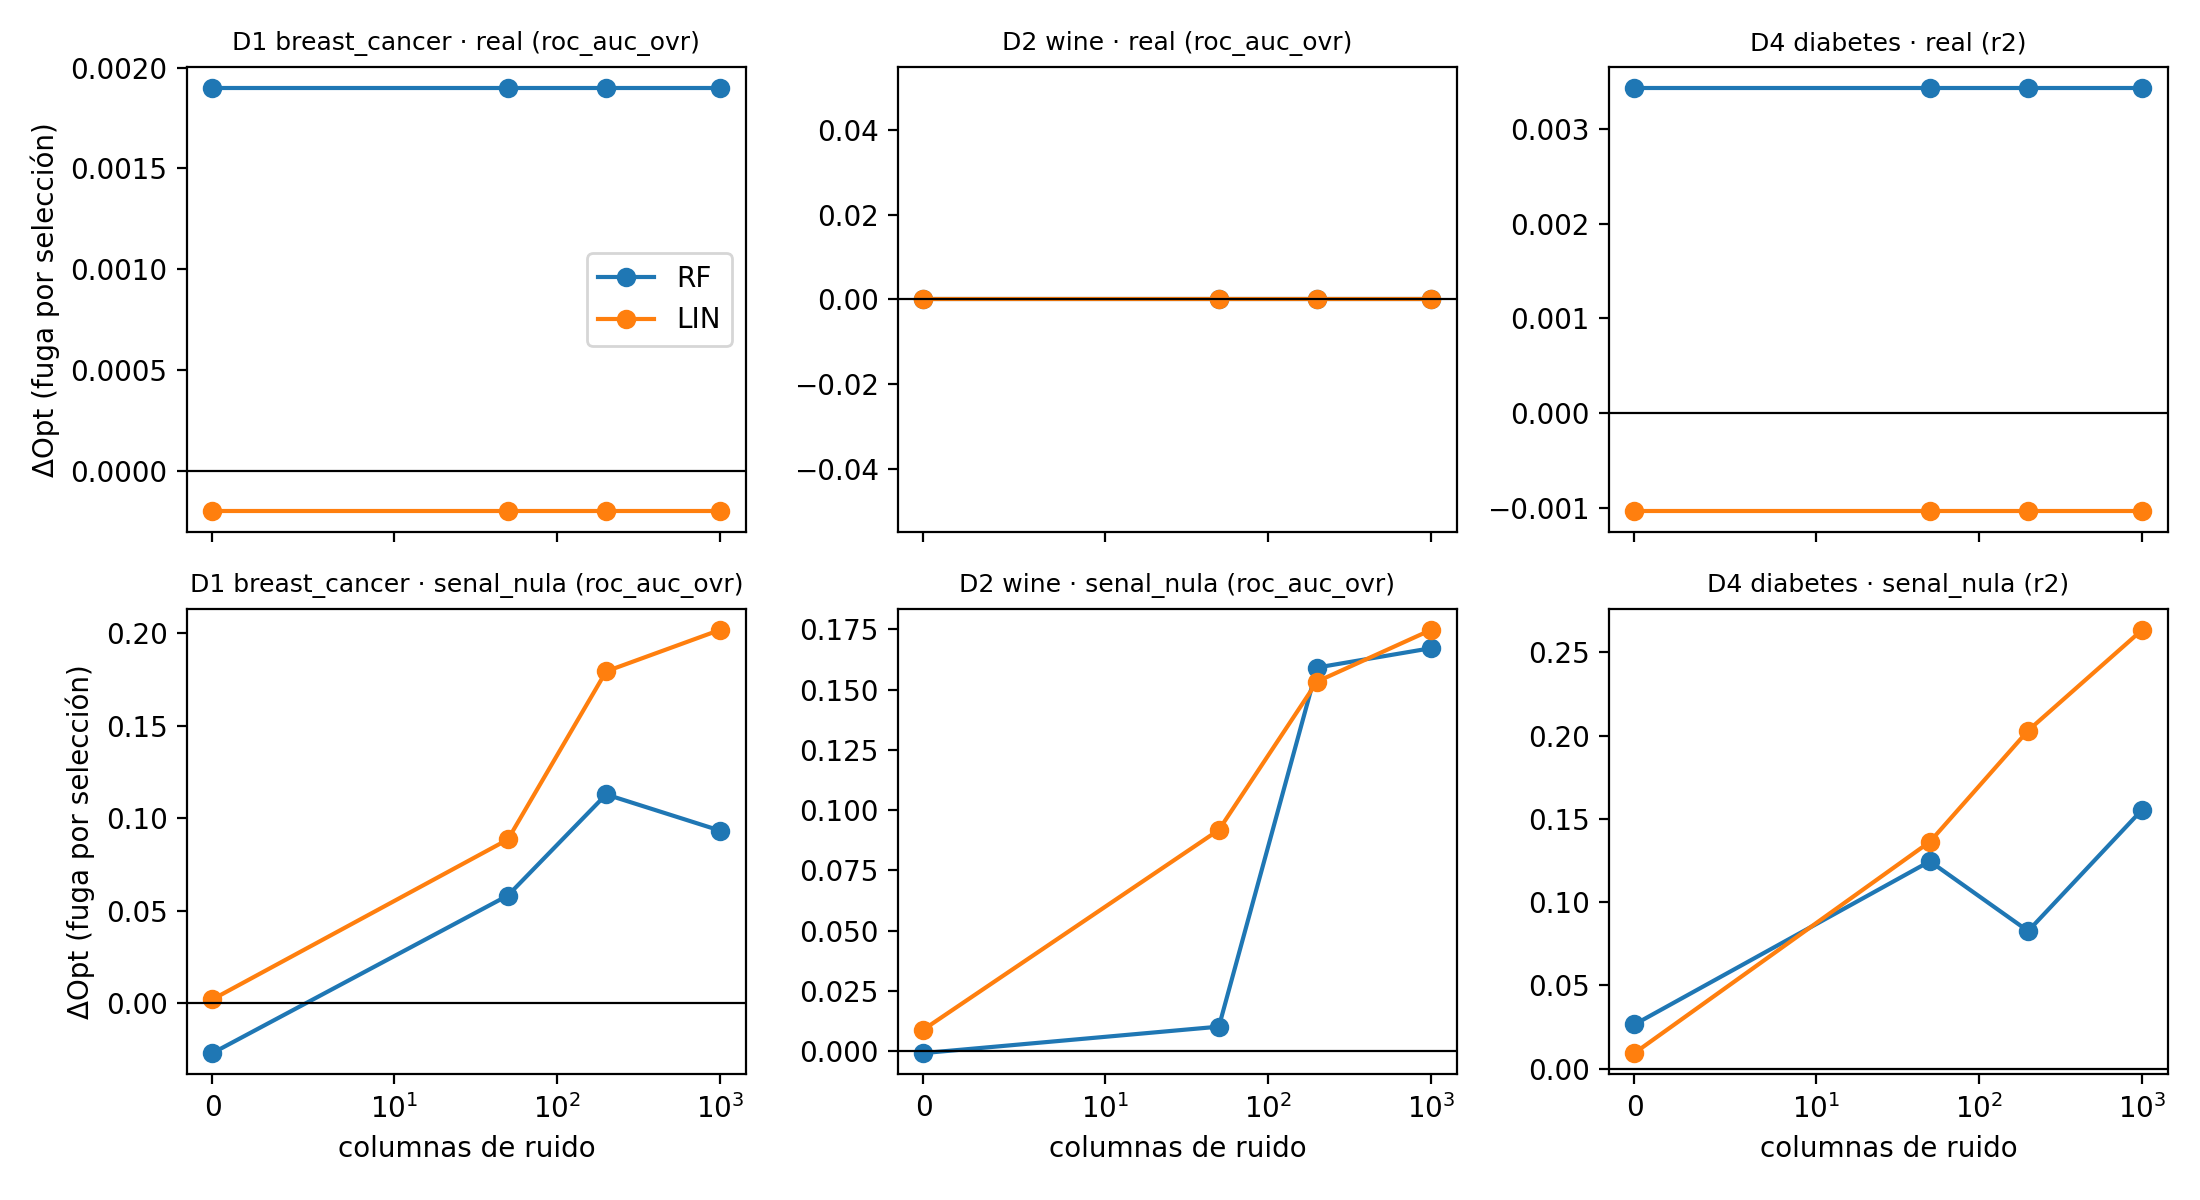
\includegraphics[width=0.95\textwidth]{fig_noise_sensitivity.png}
\caption{\DOpt{} de la selección con fuga según el número de columnas de ruido. Fila superior: etiquetas reales. Fila inferior: señal nula (control positivo).}
\label{fig:ruido}
\end{figure}

Con etiquetas reales, \DOpt{} \textbf{no cambia} con el ruido (por ejemplo, \texttt{breast\_cancer} con RandomForest: 0,0019 en los cuatro niveles), porque con al menos 8 variables muy informativas el selector nunca elige columnas de ruido. Con señal nula crece con el ruido hasta \textbf{$+0{,}20$ de AUC} (\texttt{breast\_cancer}, lineal, 1000 columnas) y \textbf{$+0{,}26$ de $R^2$} (\texttt{diabetes}, lineal): el selector «encuentra» columnas de ruido que, por azar, parecen predecir.
